\chapter{Centrale krachten: planeten en satellieten}\label{ch:b1:central-forces}

Eenendertig satellieten draaien twee keer per dag om de aarde, elk een klok
en een radiozender, en een telefoon die er vier hoort weet tot op enkele meters
waar zij is. De komeet van Halley valt achtendertig jaar lang naar de zon,
zwaait er in een paar weken omheen en klimt er weer achtendertig jaar vandaan.
Een sonde op weg naar Mars verlaat de aarde met precies de snelheid die haar
\omterm{def:b1:point-kinematics:frame}{baan} de \omterm{def:b1:point-kinematics:frame}{baan} van Mars laat raken. Dit alles is de beweging van een lichaam dat
naar een vast punt wordt aangetrokken door een kracht die afneemt als het
omgekeerde kwadraat van de afstand, en het volgt alles uit twee behouden
grootheden --- energie en \omterm{def:b1:angular-momentum:L}{impulsmoment} --- plus één nieuw idee, de effectieve
potentiaal. Dit hoofdstuk leidt de vormen en de snelheden van de banen af, de
drie \omterm{thm:b1:central-forces:conics}{wetten van Kepler}, en het rekenwerk om een satelliet te zetten waar men
hem hebben wil.

\section{Centrale conservatieve krachten}

\begin{definition}[Centrale kracht; centrale conservatieve kracht]\label{def:b1:central-forces:central}
\index{centrale kracht}\index{effectieve potentiële energie}
Een kracht heet \emph{centraal} met centrum $O$ als zij altijd langs
$\vect{OM}$ is gericht: $\vect F = F(M)\,\vect e_r$. Zij is \emph{centraal
conservatief} als haar grootte alleen van $r = OM$ afhangt: $\vect F =
F(r)\,\vect e_r$, wat afgeleid wordt van een \omterm{def:b1:work-and-energy:conservative}{potentiële energie} $E_p(r)$ met
$F(r) = -\dd E_p/\dd r$.
\end{definition}

\begin{theorem}[Beweging onder een centrale conservatieve kracht]\label{thm:b1:central-forces:reduction}
\index{perkenwet}
Een \omterm{def:b1:point-kinematics:frame}{puntmassa} met massa $m$ die alleen aan een centrale \omterm{def:b1:work-and-energy:conservative}{conservatieve kracht} is onderworpen:
\begin{enumerate}
  \item behoudt haar \omterm{def:b1:angular-momentum:L}{impulsmoment} $\vect L_O$; haar beweging is vlak en,
        in \omterm{def:b1:point-kinematics:cylindrical}{poolcoördinaten} in dat vlak, is $r^2\dot\theta = C$
        constant (\omterm{cor:b1:angular-momentum:central}{perkenwet}, \cref{cor:b1:angular-momentum:central});
  \item behoudt haar \omterm{thm:b1:work-and-energy:em}{mechanische energie} $E_m = \tfrac12 m(\dot r^2 + r^2\dot\theta^2)
        + E_p(r)$, die te schrijven is als
        \[
        E_m = \tfrac12 m\dot r^2 + E_{p,\mathrm{eff}}(r), \qquad
        E_{p,\mathrm{eff}}(r) = E_p(r) + \frac{mC^2}{2r^2} = E_p(r) + \frac{L^2}{2mr^2} .
        \]
\end{enumerate}
De radiale beweging is dus die van een eendimensionale massa in de
\emph{effectieve potentiaal} $E_{p,\mathrm{eff}}$: de radiale \omterm{def:b1:work-and-energy:turning}{keerpunten}
zijn de wortels van $E_{p,\mathrm{eff}}(r) = E_m$, de beweging is
gebonden als zij tussen twee daarvan gevangen zit, en cirkelvormig als $r$ in
een minimum van $E_{p,\mathrm{eff}}$ ligt.
\end{theorem}

\begin{proof}
Punt 1 is \cref{cor:b1:angular-momentum:central}. De kracht is
conservatief en er werkt geen andere kracht, dus blijft $E_m$ behouden; in het
vlak is $v^2 = \dot r^2 + r^2\dot\theta^2$ en $r^2\dot\theta^2 = C^2/r^2$.
De term $mC^2/2r^2$, de \omterm{thm:b1:work-and-energy:ke}{kinetische energie} van de hoekbeweging, werkt in het
radiale probleem als een afstotende \emph{\omterm{prop:b1:central-forces:effective}{centrifugale barrière}}, waarop de
eendimensionale analyse van \cref{ch:b1:work-and-energy} van toepassing is.
\end{proof}

\section{Newtoniaanse gravitatie}

\begin{definition}[Universele gravitatie]\label{def:b1:central-forces:gravitation}
\index{gravitatie}\index{gravitationele potentiële energie}
Een \omterm{def:b1:point-kinematics:frame}{puntmassa} $M$ in $O$ trekt een \omterm{def:b1:point-kinematics:frame}{puntmassa} $m$ in $M$ aan met
\[
\vect F = -\frac{GMm}{r^2}\,\vect e_r, \qquad E_p = -\frac{GMm}{r} \quad (E_p \to 0 \text{ in het oneindige}),
\]
$G = \qty{6.67e-11}{N.m^2/kg^2}$. Een bolsymmetrisch lichaam trekt buiten
zichzelf aan alsof zijn massa in zijn middelpunt zat (aangenomen; een
gevolg van de stelling van Gauss, \cref{ch:b1:electrostatics-gauss}).
\end{definition}

\begin{proposition}[De effectieve potentiaal van de gravitatie]\label{prop:b1:central-forces:effective}
\index{centrifugale barrière}\index{cirkelbaan}
Voor $E_p = -GMm/r$ is
\[
E_{p,\mathrm{eff}}(r) = -\frac{GMm}{r} + \frac{L^2}{2mr^2}
\]
gelijk aan $+\infty$ in de limiet $r \to 0$ (bij $L \neq 0$), aan $0^-$ in het oneindige,
en heeft zij één minimum in $r_c = L^2/GMm^2$, met waarde $-G^2M^2m^3/2L^2$.
Dus: $E_m < 0$ --- \omterm{def:b1:work-and-energy:turning}{gebonden beweging} tussen een kleinste en een grootste
straal (perigeum en apogeum); $E_m \geq 0$ --- ongebonden, het lichaam komt
uit het oneindige en keert erheen terug; $E_m$ gelijk aan het minimum --- cirkelbaan
met straal $r_c$.
\end{proposition}

\begin{proof}
De limieten zijn af te lezen; $E_{p,\mathrm{eff}}' = GMm/r^2 - L^2/mr^3 = 0$ in
$r_c$; invullen. Het cirkelvormige geval is $\dot r = 0$ voor altijd, en dat kan
alleen in het minimum.
\end{proof}

\begin{omfigure}
\begin{tikzpicture}
\begin{axis}[omaxis, axis x line=bottom, axis y line=left, width=10.5cm, height=6cm, xlabel={$r/r_c$}, ylabel={$E_{p,\mathrm{eff}}$},
    xlabel style={at={(axis description cs:0.5,-0.06)}, anchor=north},
    xmin=0, xmax=6, ymin=-1.2, ymax=1.2, xtick={1,2,3,4,5}, ytick={-1,0,1}, yticklabels={$-\frac{GMm}{2r_c}$,$0$,}]
  \addplot[omDef, thick, domain=0.36:6, samples=300] {-2/x + 1/x^2};
  \addplot[omExo, dashed, domain=0:6, samples=2] {0};
  \addplot[omThm, dashed, domain=0:6, samples=2] {-0.5};
  \addplot[omProp, dashed, domain=0:6, samples=2] {0.4};
  \draw[Stealth-Stealth, omThm] (axis cs:0.586,-0.5) -- (axis cs:3.41,-0.5);
  \node[omThm, font=\footnotesize, above] at (axis cs:2.0,-0.48) {$E_m < 0$: ellips};
  \node[omProp, font=\footnotesize, above] at (axis cs:3.5,0.42) {$E_m > 0$: hyperbool};
  \node[omExo, font=\footnotesize, above] at (axis cs:4.8,0.02) {$E_m = 0$: parabool};
  \fill[omDef] (axis cs:1,-1) circle (1.5pt); \node[omDef, font=\footnotesize, right] at (axis cs:1.15,-1.0) {cirkelvormig};
  \node[font=\footnotesize, omDef] at (axis cs:0.9,0.8) {$\dfrac{L^2}{2mr^2}$};
  \node[font=\footnotesize, omDef] at (axis cs:5.2,-0.72) {$-\dfrac{GMm}{r}$};
\end{axis}
\end{tikzpicture}

{\small De effectieve potentiaal van de newtoniaanse \omterm{def:b1:central-forces:gravitation}{gravitatie}: de
aantrekking $-GMm/r$ plus de \omterm{prop:b1:central-forces:effective}{centrifugale barrière} $L^2/2mr^2$. Onder
energie nul zit de radiale beweging gevangen tussen twee \omterm{def:b1:work-and-energy:turning}{keerpunten}
(perigeum, apogeum); in het minimum is de \omterm{def:b1:point-kinematics:frame}{baan} cirkelvormig; bij of boven
nul ontsnapt het lichaam.}
\end{omfigure}

\begin{theorem}[Cirkelbanen]\label{thm:b1:central-forces:circular}
\index{baansnelheid}\index{derde wet van Kepler}
Op een cirkelbaan met straal $r$ om een massa $M$:
\[
v = \sqrt{\frac{GM}{r}}, \qquad
T = 2\pi\sqrt{\frac{r^3}{GM}}, \qquad
E_m = -\frac{GMm}{2r} = -E_k = \tfrac12 E_p .
\]
In het bijzonder is $T^2/r^3 = 4\pi^2/GM$ hetzelfde voor alle cirkelbanen
om hetzelfde centrum (de \omterm{thm:b1:central-forces:circular}{derde wet van Kepler}).
\end{theorem}

\begin{proof}
Een eenparige cirkelbeweging vergt de \omterm{prop:b1:newton-dynamics:centripetal}{centripetale kracht} $mv^2/r = GMm/r^2$;
$T = 2\pi r/v$; $E_k = \tfrac12 mv^2 = GMm/2r$ en $E_p = -GMm/r$.
\end{proof}

\begin{example}[Drie banen]\label{ex:b1:central-forces:orbits}
$GM_\oplus = \qty{3.99e14}{m^3/s^2}$. Lage \omterm{def:b1:point-kinematics:frame}{baan} ($r = \qty{6770}{km}$,
\qty{400}{km} hoog): $v = \qty{7.7}{km/s}$, $T = \qty{92}{min}$. Geostationair
($T = \qty{86164}{s}$, één sterrendag): $r = (GMT^2/4\pi^2)^{1/3} =
\qty{42200}{km}$, $v = \qty{3.1}{km/s}$. De maan ($r = \qty{384000}{km}$):
$T = \qty{27.4}{d}$ --- en haar \omterm{cor:b1:point-kinematics:circular}{centripetale versnelling} $v^2/r =
\qty{2.7e-3}{m/s^2}$ is $g/3600$ op zestig aardstralen: het omgekeerde
kwadraat, door Newton zelf nagerekend.
\end{example}

\section{De wetten van Kepler en de vorm van de banen}

\begin{theorem}[Banen in een newtoniaans veld]\label{thm:b1:central-forces:conics}
\index{wetten van Kepler}\index{kegelsnede}\index{ellips (baan)}\index{excentriciteit}
De \omterm{def:b1:point-kinematics:frame}{baan} van een lichaam in het veld van een vaste massa $M$ is een kegelsnede
met $O$ in een \omterm{def:b1:mirrors-thin-lenses:mirror}{brandpunt}: een ellips als $E_m < 0$, een parabool als $E_m = 0$,
een hyperbool als $E_m > 0$. Voor de ellips met halve lange as $a$ en
excentriciteit $e$:
\begin{itemize}
  \item (Kepler I) het krachtcentrum ligt in een \omterm{def:b1:mirrors-thin-lenses:mirror}{brandpunt}; perigeum en apogeum
        liggen bij $r_p = a(1 - e)$ en $r_a = a(1 + e)$;
  \item (Kepler II) de perksnelheid is constant (de \omterm{cor:b1:angular-momentum:central}{perkenwet});
  \item (Kepler III) de omlooptijd voldoet aan $T^2 = 4\pi^2a^3/GM$;
  \item de energie hangt alleen van $a$ af, $E_m = -GMm/2a$, zodat de
        snelheid op afstand $r$ gegeven wordt door
        \[
        v^2 = GM\left(\frac{2}{r} - \frac{1}{a}\right) .
        \]
\end{itemize}
\end{theorem}
\admitted

\begin{remark}[Wat bewezen is en wat wordt aangenomen]\label{rem:b1:central-forces:admitted}
Kepler II en de indeling naar energie zijn hierboven bewezen. Dat de
gebonden banen precies ellipsen zijn met $O$ in een \omterm{def:b1:mirrors-thin-lenses:mirror}{brandpunt}, met Kepler III
en $E_m = -GMm/2a$ in het algemeen, vergt de integratie van de radiale
vergelijking (het volume van jaar 2 doet dat); voor cirkelbanen ($a = r$,
$e = 0$) valt elke uitspraak terug op \cref{thm:b1:central-forces:circular},
en dat is de controle die wij hier kunnen uitvoeren. De betrekking $v^2 = GM(2/r - 1/a)$
volgt uit $E_m = \tfrac12 mv^2 - GMm/r = -GMm/2a$ zodra die
energieformule is toegegeven.
\end{remark}

\begin{omfigure}
\begin{tikzpicture}[font=\small, x=1cm, y=1cm]
  % ellipse a=3, e=0.6, c=1.8, b=2.4 ; focus O at origin ; center at (-1.8,0)
  \draw[omDef, thick] (-1.8,0) ellipse (3 and 2.4);
  \fill (0,0) circle (1.8pt) node[below] {$O$};
  \fill (-3.6,0) circle (1.2pt) node[below] {$O'$};
  \draw[dashed] (-4.8,0) -- (1.2,0);
  \fill[omThm] (1.2,0) circle (1.6pt) node[below right] {$P$};
  \fill[omThm] (-4.8,0) circle (1.6pt) node[below left] {$A$};
  \draw[Stealth-Stealth, omExo] (-1.8,-2.6) -- (1.2,-2.6) node[midway, below] {$a$};
  \draw[Stealth-Stealth, omExo] (-1.8,0.1) -- (-1.8,2.4) node[midway, left] {$b$};
  \draw[Stealth-Stealth, omExo] (-1.8,0.45) -- (0,0.45) node[midway, above] {$c = ea$};
  \node[omThm, font=\footnotesize] at (0.7,0.8) {$r_p = a(1 - e)$};
  \node[omThm, font=\footnotesize] at (-3.4,0.8) {$r_a = a(1 + e)$};
  % hyperbola and parabola sketches on the right
  \begin{scope}[xshift=6.3cm]
  \fill (0,0) circle (1.8pt) node[below] {$O$};
  \draw[omProp, thick, domain=-1.55:1.55, samples=80, variable=\t] plot ({1.0*cosh(\t)-1.6},{1.2*sinh(\t)});
  \draw[omExo, thick, domain=-2.4:2.4, samples=80, variable=\y] plot ({0.5*\y*\y-2.6},{\y});
  \node[omProp, font=\footnotesize] at (0.0,2.9) {$E_m > 0$};
  \node[omExo, font=\footnotesize] at (-2.2,2.9) {$E_m = 0$};
  \end{scope}
\end{tikzpicture}

{\small Links: een elliptische \omterm{def:b1:point-kinematics:frame}{baan} om het \omterm{def:b1:mirrors-thin-lenses:mirror}{brandpunt} $O$ --- halve lange
as $a$, halve korte as $b$, \omterm{def:b1:mirrors-thin-lenses:lens}{brandpuntsafstand} $c = ea$; het lichaam is het snelst in
het perigeum $P$ en het traagst in het apogeum $A$. Rechts: een hyperbool (positieve
energie) en een parabool (energie nul) om hetzelfde \omterm{def:b1:mirrors-thin-lenses:mirror}{brandpunt} --- de ongebonden
banen van kometen en sondes.}
\end{omfigure}

\begin{example}[De komeet van Halley]\label{ex:b1:central-forces:halley}
Perihelium \qty{0.586}{AU}, aphelium \qty{35.1}{AU}: $a = \qty{17.8}{AU}$,
$e = 0.967$, $T = \sqrt{17.8^3} = \qty{75}{jaar}$ (Kepler III in
astronomische eenheden en jaren, waar $T^2 = a^3$ geldt voor de zon). Met
$GM_\odot = \qty{1.33e20}{m^3/s^2}$ is de snelheid in het perihelium
$\sqrt{GM(2/r_p - 1/a)} = \qty{54}{km/s}$ en in het aphelium \qty{0.9}{km/s}
--- zestig keer trager, zoals de \omterm{cor:b1:angular-momentum:central}{perkenwet} eist ($r_pv_p = r_av_a$).
\end{example}

\section{Satellieten}

\begin{proposition}[Ontsnappingssnelheid; geostationaire baan]\label{prop:b1:central-forces:escape}
\index{ontsnappingssnelheid}\index{geostationaire baan}
Vanaf het oppervlak van een lichaam met massa $M$ en straal $R$ is de kleinste
lanceersnelheid om het oneindige te bereiken $v_e = \sqrt{2GM/R} = \sqrt2\,v_c$,
waarin $v_c = \sqrt{GM/R}$ de cirkelsnelheid aan de grond is:
\qty{11.2}{km/s} voor de aarde. Een \emph{geostationaire} satelliet draait
in het vlak van de evenaar mee met de sterrendag van de aarde, op
$r = \qty{42200}{km}$ (\qty{35800}{km} boven de grond).
\end{proposition}

\begin{proof}
$E_m \geq 0$: $\tfrac12 mv_e^2 - GMm/R = 0$. Kepler III met $T = \qty{86164}{s}$.
\end{proof}

\begin{proposition}[Hohmann-transfer]\label{prop:b1:central-forces:hohmann}
\index{Hohmann-transfer}
Om een satelliet met twee korte stuwstoten van een cirkelbaan met straal $r_1$
naar een cirkelbaan met straal $r_2 > r_1$ in hetzelfde vlak te brengen: geef bij $r_1$
een stoot om de \emph{transferellips} met perigeum $r_1$ en apogeum $r_2$
($a = (r_1 + r_2)/2$) op te gaan, zweef een halve periode mee, en geef bij $r_2$
opnieuw een stoot om de \omterm{def:b1:point-kinematics:frame}{baan} cirkelvormig te maken:
\[
\Delta v_1 = \sqrt{\frac{GM}{r_1}}\left(\sqrt{\frac{2r_2}{r_1 + r_2}} - 1\right),
\qquad
\Delta v_2 = \sqrt{\frac{GM}{r_2}}\left(1 - \sqrt{\frac{2r_1}{r_1 + r_2}}\right),
\qquad
t = \pi\sqrt{\frac{(r_1 + r_2)^3}{8GM}} .
\]
\end{proposition}

\begin{proof}
De snelheden op de transferellips uit $v^2 = GM(2/r - 1/a)$ in $r_1$ en
$r_2$; trek daar de cirkelsnelheden van af; de halve omlooptijd uit
\cref{thm:b1:central-forces:conics}.
\end{proof}

\begin{omfigure}
\begin{tikzpicture}[font=\small, x=1cm, y=1cm]
  \fill (0,0) circle (2.5pt) node[below left] {$O$};
  \draw[omDef, thick] (0,0) circle (1.0);
  \draw[omDef, thick] (0,0) circle (3.0);
  % transfer ellipse: perigee r1=1 at (1,0), apogee r2=3 at (-3,0): a=2, c=1, center (-1,0), b=sqrt(3)=1.732
  \draw[omThm, thick] (-1,0) ellipse (2 and 1.732);
  \fill[omThm] (1,0) circle (1.6pt); \fill[omThm] (-3,0) circle (1.6pt);
  \draw[-Stealth, omExo, very thick] (1,0) -- (1,1.0) node[right] {$\Delta v_1$};
  \draw[-Stealth, omExo, very thick] (-3,0) -- (-3,-0.8) node[left] {$\Delta v_2$};
  \node[omDef, font=\footnotesize] at (1.5,-1.2) {$r_1$};
  \node[omDef, font=\footnotesize] at (2.6,2.3) {$r_2$};
  \node[omThm, font=\footnotesize] at (-1.0,2.0) {transferellips};
  \draw[-Stealth, omThm] (-0.2,1.72) -- (-0.8,1.73);
\end{tikzpicture}

{\small Een \omterm{prop:b1:central-forces:hohmann}{Hohmann-transfer} tussen twee cirkelbanen: een eerste stuwstoot op
de binnenste \omterm{def:b1:point-kinematics:frame}{baan} tilt het apogeum op tot $r_2$; een halve ellips later tilt een
tweede stoot het perigeum op --- de zuinigste route met twee stoten, en
die welke een sonde naar Mars brengt.}
\end{omfigure}

\begin{example}[Van lage baan naar geostationair]\label{ex:b1:central-forces:leogeo}
$r_1 = \qty{6770}{km}$, $r_2 = \qty{42200}{km}$: $\Delta v_1 = \qty{2.4}{km/s}$,
$\Delta v_2 = \qty{1.5}{km/s}$, \qty{5.3}{h} meezweven. Het totaal,
\qty{3.9}{km/s}, is de helft van wat de lancering naar de lage \omterm{def:b1:point-kinematics:frame}{baan} al kostte: de
``laatste kilometer'' naar een hoge \omterm{def:b1:point-kinematics:frame}{baan} is duur, en satellieten dragen daarvoor
hun eigen motor mee.
\end{example}

\begin{remark}[Afstotende centra]\label{rem:b1:central-forces:rutherford}
\index{Rutherford-verstrooiing}
Bij een afstotende kracht die gaat als het omgekeerde kwadraat (twee gelijknamige ladingen,
\cref{ch:b1:electrostatics-gauss}) heeft de effectieve potentiaal geen kuil:
elke \omterm{def:b1:point-kinematics:frame}{baan} is een hyperbool, het deeltje nadert, wordt afgebogen
en vertrekt weer. Richt men een $\alpha$-deeltje recht op een goudkern, dan volgt zijn
kleinste naderingsafstand alleen uit de energie, $E_k =
2Ze^2/4\pi\varepsilon_0 r_{\min}$ --- de manier waarop Rutherford de grootte van
de kern afschatte (\cref{exo:b1:central-forces:11}).
\end{remark}

\section{Oefeningen}

\begin{exercise}[$\star$]\label{exo:b1:central-forces:1}
Het internationale ruimtestation draait op \qty{400}{km} hoogte
($R_\oplus = \qty{6370}{km}$, $GM_\oplus = \qty{3.99e14}{m^3/s^2}$). Snelheid,
omlooptijd, aantal zonsopgangen dat de bemanning per dag ziet.
\end{exercise}

\begin{exercise}[$\star$]\label{exo:b1:central-forces:2}
Bepaal straal en hoogte van de \omterm{prop:b1:central-forces:escape}{geostationaire baan} uit de sterrendag
\qty{86164}{s}, en de baansnelheid.
\end{exercise}

\begin{exercise}[$\star$]\label{exo:b1:central-forces:3}
Ontsnappingssnelheid van de aarde en van de maan ($GM = \qty{4.90e12}{m^3/s^2}$,
$R = \qty{1740}{km}$). Waarom houdt de maan geen atmosfeer vast?
\end{exercise}

\begin{exercise}[$\star$]\label{exo:b1:central-forces:4}
Mars heeft $a = \qty{1.524}{AU}$, Jupiter \qty{5.20}{AU}: hun jaren, met
de \omterm{thm:b1:central-forces:circular}{derde wet van Kepler}. Een lichaam op \qty{30}{AU} (Neptunus)?
\end{exercise}

\begin{exercise}[$\star\star$]\label{exo:b1:central-forces:5}
Energie om \qty{1000}{kg} in de \omterm{def:b1:point-kinematics:frame}{baan} van het ruimtestation te brengen, vertrekkend
uit rust aan het oppervlak (verwaarloos de aardrotatie en de lucht). Vergelijk
met de chemische energie van benzine (\qty{46}{MJ/kg}).
\end{exercise}

\begin{exercise}[$\star\star$]\label{exo:b1:central-forces:6}
De komeet van Halley: perihelium \qty{0.586}{AU}, aphelium \qty{35.1}{AU}.
Bereken $a$, $e$, de omlooptijd en de snelheden in het perihelium en het aphelium
($GM_\odot = \qty{1.33e20}{m^3/s^2}$, $\qty{1}{AU} = \qty{1.496e11}{m}$).
\end{exercise}

\begin{exercise}[$\star\star$]\label{exo:b1:central-forces:7}
\omterm{prop:b1:central-forces:hohmann}{Hohmann-transfer} van de \omterm{def:b1:point-kinematics:frame}{baan} van het ruimtestation (\qty{6770}{km}) naar de
\omterm{prop:b1:central-forces:escape}{geostationaire baan} (\qty{42200}{km}): beide stuwstoten, het totaal en de duur.
\end{exercise}

\begin{exercise}[$\star\star$]\label{exo:b1:central-forces:8}
Toon aan dat het minimum van $E_{p,\mathrm{eff}}$ in $r_c = L^2/GMm^2$ ligt,
en dat kleine radiale trillingen eromheen de \omterm{def:b1:wave-propagation:signal}{hoekfrequentie}
$\sqrt{GM/r_c^3}$ hebben --- de omloopfrequentie zelf. Wat zegt dat
over een licht verstoorde cirkelbaan?
\end{exercise}

\begin{exercise}[$\star\star$]\label{exo:b1:central-forces:9}
Astronauten aan boord van het ruimtestation zweven. Verklaar dat met de krachten;
hoe groot is $g$ op hun hoogte, en waarom is dat niet in tegenspraak met dat
zweven?
\end{exercise}

\begin{exercise}[$\star\star\star$]\label{exo:b1:central-forces:10}
Newtons ``maanproef'': bereken de \omterm{cor:b1:point-kinematics:circular}{centripetale versnelling} van de maan uit
$r = \qty{3.84e8}{m}$ en $T = \qty{27.3}{d}$, en vergelijk haar met
$g(R/r)^2$. Trek een conclusie.
\end{exercise}

\begin{exercise}[$\star\star\star$]\label{exo:b1:central-forces:11}
Een $\alpha$-deeltje ($q = 2e$, $E_k = \qty{5.0}{MeV}$) wordt recht op een
goudkern ($Z = 79$) afgeschoten, die vast wordt verondersteld. Bepaal met behoud
van energie en $E_p = 2Ze^2/4\pi\varepsilon_0r$ ($1/4\pi\varepsilon_0 = \qty{8.99e9}{SI}$)
de kleinste naderingsafstand; vergelijk die met de kernstraal,
ongeveer \qty{7}{fm}. Welke energie zou nodig zijn om de kern te raken?
\end{exercise}

\begin{exercise}[$\star\star\star$]\label{exo:b1:central-forces:12}
Een satelliet in een lage \omterm{def:b1:point-kinematics:frame}{baan} wordt afgeremd door de resterende atmosfeer, zodat
zijn \omterm{thm:b1:work-and-energy:em}{mechanische energie} afneemt. Toon met $E_m = -GMm/2r$ en
$v = \sqrt{GM/r}$ aan dat hij daardoor \emph{sneller} gaat. Waar blijft de
energie, en welk deel van de verloren \omterm{def:b1:work-and-energy:conservative}{potentiële energie} wordt warmte?
\end{exercise}

\begin{omfigure}
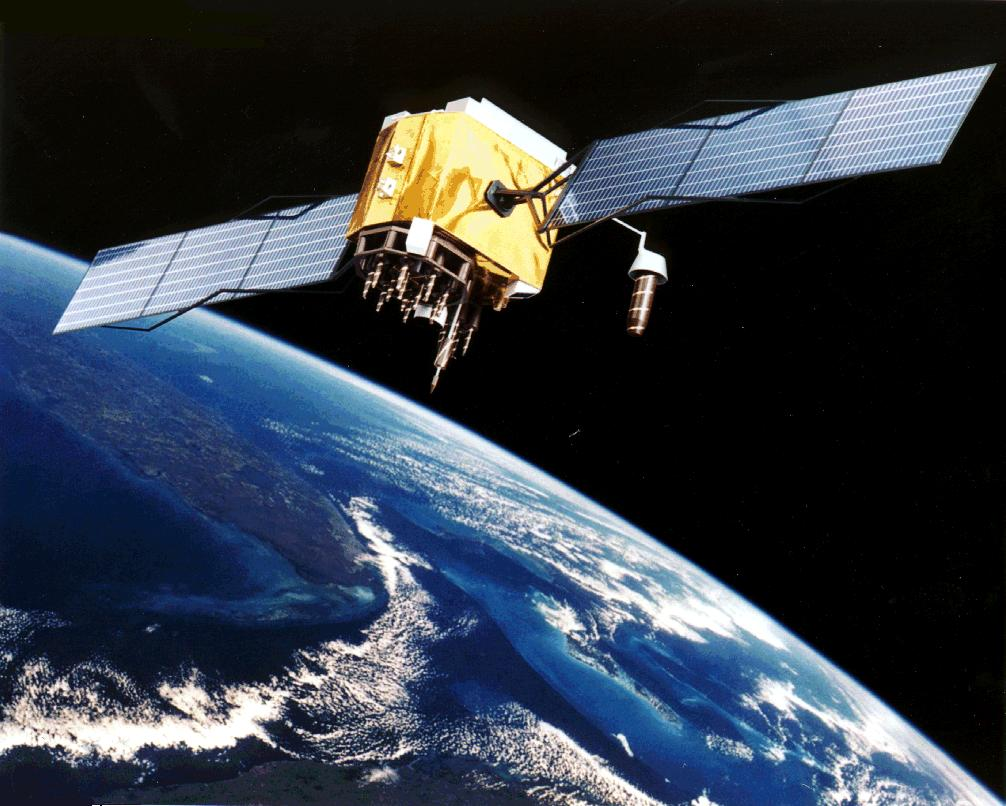
\includegraphics[width=0.46\linewidth]{images/book3/gps-satellite-nasa.jpg}

{\small Een GPS-satelliet (impressie van NASA): een van de ruim dertig in de constellatie op \qty{20200}{km} uit de weekendopgave, elk een klok in een keplerbaan.}
\end{omfigure}

\section{Probleem: De satellieten die je vertellen waar je bent}

\begin{problem}[{Weekendopgave --- een navigatieconstellatie twintigduizend
kilometer hoog: haar baan, de brandstof om er te komen, hoeveel
satellieten een telefoon ziet, en waarom hun klokken opzettelijk te
langzaam moeten lopen}]
\label{pb:b1:central-forces:1}
Gegevens: $GM_\oplus = \qty{3.986e14}{m^3/s^2}$, $R_\oplus = \qty{6371}{km}$,
sterrendag \qty{86164}{s}, $c = \qty{2.998e8}{m/s}$. De satellieten
draaien in precies een halve sterrendag op cirkelbanen om de aarde.

\medskip
\noindent\textbf{Deel I --- De \omterm{def:b1:point-kinematics:frame}{baan}.}
\begin{enumerate}
  \item Bereken de straal van de \omterm{def:b1:point-kinematics:frame}{baan} en de hoogte.
  \item Bereken de baansnelheid.
  \item Bereken de versnelling van de satelliet en vergelijk haar met $g$ aan
        het oppervlak.
  \item Bereken de \omterm{thm:b1:work-and-energy:em}{mechanische energie} per kilogram, en het kinetische en het
        potentiële deel.
  \item Waarom een halve sterrendag en niet een halve zonnedag? Wat ziet een
        waarnemer op de grond zich herhalen?
  \item Onder welke hoek ziet men vanaf een satelliet de schijf van de aarde?
  \item Vergelijk de straal van deze \omterm{def:b1:point-kinematics:frame}{baan} met die van de geostationaire; welke
        ligt hoger, en met welke factor?
\end{enumerate}

\medskip
\noindent\textbf{Deel II --- Erheen komen.}
\begin{enumerate}[resume]
  \item Energie per kilogram om van rust aan het oppervlak naar de eindbaan
        te gaan (verwaarloos de lucht en de aardrotatie).
  \item De draagraket bereikt eerst een lage cirkelbaan op \qty{400}{km}.
        Snelheid daar?
  \item \omterm{prop:b1:central-forces:hohmann}{Hohmann-transfer} van die \omterm{def:b1:point-kinematics:frame}{baan} naar de eindbaan: de twee stuwstoten
        en hun som.
  \item Duur van de transfer.
  \item Vergelijk de som van de stoten met de ontsnappingssnelheid vanuit de lage
        \omterm{def:b1:point-kinematics:frame}{baan}: hoe ver is deze vlucht van ``de aarde verlaten''?
  \item Bovenste trap en satelliet wegen samen \qty{2000}{kg} vóór de
        transfer; de uitstroomsnelheid van de motor is \qty{3.0}{km/s} en de
        raketvergelijking geeft $\Delta v = u\ln(m_0/m_1)$. Hoeveel stuwstof
        vergen de twee stoten?
\end{enumerate}

\medskip
\noindent\textbf{Deel III --- Dekking en tijdmeting.}
\begin{enumerate}[resume]
  \item Een satelliet is zichtbaar vanuit elk punt van de aarde dat binnen
        de kegel met halve tophoek $\theta$ ligt, waarbij $\cos\theta = R/r$,
        om de lijn aarde--satelliet. Bereken $\theta$ en het
        deel $(1 - \cos\theta)/2$ van het aardoppervlak dat hij bestrijkt.
  \item Met $24$ gelijkmatig verdeelde satellieten: hoeveel zijn er gemiddeld
        zichtbaar vanuit één punt? Is het minimum van $4$ dat een
        plaatsbepaling vergt aannemelijk?
  \item Looptijd van het licht vanaf een satelliet in het zenit; aan de
        horizon.
  \item Om de ontvanger tot op \qty{3}{m} te plaatsen: met welke
        nauwkeurigheid moet de aankomsttijd van de signalen worden gemeten?
  \item De klok van de ontvanger zelf is goedkoop kwarts en wijkt
        milliseconden af: waarom zijn er vier satellieten nodig in plaats van drie?
  \item De klokken van de satellieten zijn atoomklokken. Geef de relatieve
        stabiliteit die nodig is voor een fout van \qty{3}{m} na één dag.
\end{enumerate}

\medskip
\noindent\textbf{Deel IV --- Kort over relativiteit.}
Twee effecten verschuiven de satellietklokken ten opzichte van klokken op de
grond (formules aangenomen, uit het volume van jaar 3): beweging vertraagt een
klok met het deel $v^2/2c^2$; hoogte versnelt haar met $GM(1/R - 1/r)/c^2$.
\begin{enumerate}[resume]
  \item Bereken de vertraging door de snelheid, in microseconden per dag.
  \item Bereken de versnelling door de hoogte, in microseconden per
        dag.
  \item Het netto-effect, en de plaatsfout die het per dag zou geven als het
        niet werd gecorrigeerd.
  \item De satellietklokken worden vóór de lancering op
        \qty{10.22999999543}{MHz} gezet in plaats van \qty{10.23}{MHz}. Ga na
        dat dit het netto-effect compenseert.
  \item De banen zijn niet precies keplerbanen: noem drie storingen
        en zeg hoe het systeem daarmee omgaat.
  \item Vat de keten samen: twee behoudswetten, één \omterm{def:b1:point-kinematics:frame}{baan}, één
        constellatie, en de ene correctie die niemand had verwacht.
\end{enumerate}
\end{problem}
